\documentclass{iopart}
\usepackage{amssymb}
\usepackage{graphicx}
\usepackage{algorithmic}
\usepackage{algorithm}
\usepackage{url}
\usepackage{color}
%\usepackage{hyperref}
\newcommand{\mbf}[1]{\mathbf{#1}}
\newcommand{\mcl}[1]{\mathcal{#1}}
\newcommand{\msf}[1]{\mathsf{#1}}
\newcommand{\TODO}[1]{{\textcolor{red}{TODO: #1}}}
%\newcommand{\argmin}{\operatornamewithlimits{arg min}}
\newcommand{\argmin}{\mathrm{arg min}}
\newcommand{\ts}[1]{{\textstyle#1}}

\newcommand{\bq}{\begin{eqnarray}}
\newcommand{\eq}{\end{eqnarray}}
\newcommand{\diag}{\mathrm{diag}}

\newtheorem{theorem}{Theorem}[section]
\newtheorem{lemma}[theorem]{Lemma}
\newtheorem{proposition}[theorem]{Proposition}
\newtheorem{corollary}[theorem]{Corollary}

\newenvironment{proof}[1][Proof]{\begin{trivlist}
\item[\hskip \labelsep {\bfseries #1}]}{\end{trivlist}}
\newenvironment{definition}[1][Definition]{\begin{trivlist}
\item[\hskip \labelsep {\bfseries #1}]}{\end{trivlist}}
\newenvironment{example}[1][Example]{\begin{trivlist}
\item[\hskip \labelsep {\bfseries #1}]}{\end{trivlist}}
\newenvironment{remark}[1][Remark]{\begin{trivlist}
\item[\hskip \labelsep {\bfseries #1}]}{\end{trivlist}}

\newcommand{\qed}{\nobreak \ifvmode \relax \else
      \ifdim\lastskip<1.5em \hskip-\lastskip
      \hskip1.5em plus0em minus0.5em \fi \nobreak
      \vrule height0.75em width0.5em depth0.25em\fi}




\begin{document}

\title[A penalty method for PDE-constrained optimization]{A penalty method for PDE-constrained optimization}
\author{Tristan van Leeuwen$^1$ and Felix J. Herrmann$^2$}
\address{$^1$Centrum Wiskunde \& Informatica. Science Park, Amsterdam, the Netherlands\\
$^2$ Dept. of Earth, Ocean and Atmospheric Sciences.\\2207 Main Mall, Vancouver, BC Canada V6T 1Z4.}
\ead{tleeuwen@eos.ubc.ca}

\begin{abstract}
We present a method for solving PDE constrained optimization problems
based on a penalty formulation. This method aims to combine advantages
of both full-space and reduced methods by exploiting a large
search-space (consisting of both control and state variables) while
allowing for an efficient implementation that avoids storing and
updating the state-variables. This leads to a method that has roughly
the same per-iteration complexity as conventional reduced approaches
while defining an objective that is less non-linear in the control
variable by implicitly relaxing the constraint. We apply the method to a
seismic inverse problem where it leads to a particularly efficient
implementation when compared to a conventional reduced approach as it
avoids the use of adjoint state-variables. Numerical examples illustrate
the approach and suggest that the proposed formulation can indeed
mitigate some of the well-known problems with local minima in the
seismic inverse problem.
\end{abstract}

\maketitle

\section{Introduction}
In parameter estimation, the goal is to infer physical parameters (e.g., density, soundspeed or conductivity) 
from partial measurements of solutions of a PDE that describes the physical process as a 
function of the paramater of interest (e.g., a wave-equation, ). These problems arise in many applications such as
geophysics \cite{Haber2004,Epanomeritakis08}, medical imaging \cite{Abdoulaev2005} and non-destructive testing.

For linear PDEs, the resulting optimzation problem (after discretization) can be written as
\bq
\label{eq:constr}
\min_{\mbf{m},\mbf{u}} \ts{\frac{1}{2}}||P^T\mathbf{u} - \mathbf{d}||_2^2 \quad 
\mbox{s.t.} \quad A(\mathbf{m})\mathbf{u} = \mathbf{q},
\eq
where $\mathbf{m}$ is the (gridded) parameter of interest, $\mathbf{u}$ is the field and $\mathbf{d}$ are
the input data. The measurement process is modelled by taking inner products of the field with the columns of $P$. 
The matrix $A(\mathbf{m})\mathbf{u} = \mathbf{q}$ represents the discretized PDE and $\mbf{q}$ is the 
source function. 

Oftentimes, measurements are made from multiple independent experiments, 
in which case $\mathbf{u}$ is a block vector containing the fields for different experiments. 
For some applications, such as seismic inversion, $\mbf{m}$ may represent up to $\mcl{O}(10^9)$ unknowns 
while $\mbf{u}$ may easily represent $\mcl{O}(10^{17})$.

\subsection{All-at-once approach}
A popular approach to solving
these constrained problems is based on the corresponding Lagrangian:
\bq
\mcl{L}(\mbf{m},\mbf{u},\mbf{v})=  \ts{\frac{1}{2}}||P^T\mathbf{u} - \mathbf{d}||_2^2 
+ \mbf{v}^T\left(A(\mathbf{m})\mathbf{u} - \mathbf{q}\right),
\eq
where $^T$ denotes the (complex-conjugate) transpose.
A necessary condition for a solution to the constrained problem (\ref{eq:constr}) is that 
it is a stationary point of the Lagrangian. 
Such a stationary point may be found using a Newton-like method by repeatedly solving
the KKT system \cite{Haber2000}
\bq
\left(
\begin{array}{ccc}
R&K^T&G^T\\
K&PP^T&A^T\\
G&A&\\
\end{array}
\right)
\left(
\begin{array}{c}
\delta \mbf{m}\\
\delta \mbf{u}\\
\delta \mbf{v}\\
\end{array}
\right)=
-\left(
\begin{array}{c}
\mcl{L}_{\mbf{m}}\\
\mcl{L}_{\mbf{u}}\\
\mcl{L}_{\mbf{v}}\\
\end{array}
\right),
\eq
where
\bq
\mcl{L}_{\mbf{m}} &=& G(\mbf{m},\mbf{u})^T\mathbf{v},\\
\mcl{L}_{\mbf{u}} &=& A(\mathbf{m})^T\mathbf{v} + P(P^T\mathbf{u} - \mathbf{d}),\\
\mcl{L}_{\mbf{v}} &=& A(\mathbf{m})\mathbf{u} - \mathbf{q},\\
\eq
and
\bq
G(\mbf{m},\mbf{u}) &=& \frac{\partial A(\mbf{m})\mbf{u}}{\partial \mbf{m}},\\
K(\mbf{m},\mbf{v}) &=& \frac{\partial A(\mbf{m})^T\mbf{v}}{\partial \mbf{m}},\\
R(\mbf{m},\mbf{u},\mbf{v}) &=& \frac{\partial G(\mbf{m},\mbf{u})^T\mbf{v}}{\partial \mbf{m}}.
\eq
These Jacobian matrices are typically sparse and can be computed analytically.

An advantages of such an `all-at-once' approach are that it eliminates the need to
solve the PDEs explicitly. However, this approach is often unfeasible
for large-scale applications we have in mind because it involves simultaneously updating
(and hence storing) all the variables (up to $\mcl{O}(10^{17})$). 

\subsection{Reduced approach}
For large-scale applications, one usually considers a \emph{reduced} problem
\bq
\min_{\mbf{m}}\phi(\mbf{m}) = \ts{\frac{1}{2}}||P^T\mbf{u}(\mbf{m}) - \mbf{d}||_2^2,
\label{eq:redL}
\eq
where $\mbf{u}(\mbf{m}) = A(\mathbf{m})^{-1}\mathbf{q}$.
The resulting optimization problem has a much smaller dimension and can be solved using black-box 
non-linear optimization methods. The gradient and the (Gauss-Newton) Hessian of 
$\phi$ are given by

\bq
\nabla\phi(\mbf{m}) &=& G(\mbf{m},\mbf{u})^T\mbf{v},\\
\nabla^2\phi(\mbf{m}) &=& G(\mbf{m},\mbf{u})^TA(\mbf{m})^{-T}PP^TA(\mbf{m})^{-1}G(\mbf{m},\mbf{u})\nonumber\\
&& + K(\mbf{m},\mbf{v})^TA(\mbf{m})^{-T}G(\mbf{m},\mbf{u}) + G(\mbf{m},\mbf{u})^TA(\mbf{m})^{-T}K(\mbf{m},\mbf{v})\nonumber\\
&& + R(\mbf{m},\mbf{u},\mbf{v}).
\eq
where $\mbf{v} = A(\mbf{m})^{-T}P\left(\mbf{d} - P^T\mbf{u}\right)$.

The basic (Gauss-Newton) algorithm for minimizing $\phi(\mathbf{m})$ is given in 
Algorithm \ref{alg:reduced}.
\begin{algorithm}
\caption{Basic Gauss-Newton algorithm for find a stationary point of the Lagrangian via the reduced method}
\label{alg:reduced}
\begin{algorithmic}
\REQUIRE{initial guess $\mbf{m}^0$, tolerance $\epsilon$}
\STATE{$k=0$}
\REPEAT
\STATE{$\mathbf{u}^k_{\mathrm{red}}  = A(\mathbf{m}^k)^{-1}\mathbf{q}$}
\STATE{$\mathbf{v}^k_{\mathrm{red}}  = A(\mathbf{m}^k)^{-T}P(\mathbf{d} - P^T\mathbf{u}^k_{\mathrm{red}})$}
\STATE{$\mathbf{g}^k_{\mathrm{red}}    = G(\mathbf{m}^k,\mathbf{u}^k_{\mathrm{red}})^T\mathbf{v}^k_{\mathrm{red}}$}
\STATE{$H^k_{\mathrm{red}} = G(\mbf{m}^k,\mbf{u}^k_{\mathrm{red}})^TA(\mbf{m}^k)^{-T}PP^TA(\mbf{m}^k)^{-1}G(\mbf{m}^k,\mbf{u}^k_{\mathrm{red}})$}
\STATE{$\mathbf{m}^{k+1} =\mathbf{m}^k - \alpha^k \left(H_{\mathrm{red}}^{k}\right)^{-1}\mathbf{g}^k_{\mathrm{red}}$}
\UNTIL{$\|\mbf{g}_{\mathrm{red}} ^k\|_2 \leq \epsilon$}
\end{algorithmic}
\end{algorithm}
Note that this corresponds to a block-elimination of the KKT system and the iterates automatically
satisfy $\mcl{L}_{\mathbf{u}}(\mbf{m}^k,\mbf{u}^k_{\mathrm{red}},\mbf{v}^k_{\mathrm{red}}) = \mcl{L}_{\mathbf{v}}(\mbf{m}^k,\mbf{u}^k_{\mathrm{red}},\mbf{v}^k_{\mathrm{red}}) = 0$. 
If the algorithm terminates successfully, the final iterates additionally satisfy
$\|\mcl{L}_{\mathbf{m}}(\mbf{m}^*,\mbf{u}^*_{\mathrm{red}},\mbf{v}^*_{\mathrm{red}})\|_2^2 \leq \epsilon$.

The disadvantage of this approach is that it
requires the solution of the PDEs at each update, making it computationally very expensive. 
It also strictly enforces the constraint at each iteration, which might lead to a very
nonlinear problem in $\mbf{m}$. Moreover, the corresponding Hessian is typically a
dense matrix that cannot be stored and computing its action involves additional
PDE solves. Practical approaches are usually based on Quasi-Newton approximations of
the reduced Hessian.

\subsection{Contributions and outline}
In this paper we present an alternative to the reduced approach which
has a roughly equivalent per-iteration complexity in terms of PDE solves
and storage but retains some of the characteristics of the all-at-once
approach in the sense that it exploits a larger search space by not
enforcing the constraints at each iteration.

The approach is based on a \emph{penalty} formulation of the constrained problem,
the solution of which coincides with that of the constrained problem (\ref{eq:constr}) for an. 
appropriate choice of the penalty parameter.
Such a reformulations of the constrained problem are well-known, 
but for the sake of completeness we give a brief overview in section \ref{penalty}. The main contribution
of this paper is a solution strategy, which is based on the elimination of the state variable $u$ via
a \emph{variational projection} approach as detailed in section \ref{varpro}. The benefit of this approach is
that it effectively eliminates these variables from the optizatiom problem and thus greatly reduces the dimensionality
of the optimization problem. Due to the special structure of the problems under consideration, this elimination 
can be done efficiently, leading to a tractable algorith for large-scale problems. 
Contrary to the conventional \emph{reduced} approach, the resulting algorihtm does \emph{not} enforce the constraint
at each iteration and arguably leads to a less non-linear problem in $\mbf{m}$. It is outside the scope of the current
paper to give a rigorous prove of this statement, but a case-study presented in section
 \ref{examples} provides some numerical evidence.

A detailed description of the proposed algorihtm is given in section \ref{algorithm}.
Here, we also compare the penalty approach to both the all-at-once and the
reduced approaches in terms of algorithmic complexity.

Numerical
examples on seismic inversion using both the penalty and reduced
formulations are given in section \ref{examples}.

Possible extensions and open problems are discussed in section
\ref{discussion} and section \ref{conclusion} gives the conclusions.

\subsection{Related work}
The proposed method is related to the \emph{equation-error} approach,
which is typically used to identify the control variable in diffusion
problems given a \emph{complete} measurement of the state: $\mbf{d} = \mbf{u}$ by
solving $A(\mbf{m})\mbf{u} = \mbf{q}$ for $\mbf{m}$ \cite{Richter1981,Banerjee2013}. 
Given \emph{partial} measurements of the state $\mbf{d} = P^T\mbf{u}$, the proposed method can be seen as a
way of bootstrapping this by first attempting to reconstruct the complete
state from the partial measurements. 

\section{Penalty methods}
\label{penalty}
A constrained optimization problems of the form (\ref{eq:constr})
can be recast as an unconstrained problem by introducing a positive penalty function $\pi$ as follows
\bq
\label{eq:penalty}
\min_{\mbf{m},\mbf{u}} \Phi_{\lambda} = \ts{\frac{1}{2}}||P^T\mathbf{u} - \mathbf{d}||_2^2 + \lambda\pi(\mbf{A}(\mbf{m})\mbf{u} - \mbf{q}).
\eq
The idea is that any departure from the constraint is penalized so that the solution of this 
unconstrained problem will coincide with that of the constrained problem when $\lambda$ is large enough.

\subsection{Quadratic penalty function}
A quadratic penalty function $\pi(\cdot) = \ts{\frac{1}{2}}||\cdot||_2^2$ leads to a differentiable 
unconstrained optimization problem (\ref{eq:penalty}) whose minimizer $\{\overline{\mbf{m}}_{\lambda},\overline{\mbf{u}}_{\lambda}\}$ coincides with the solution
of the constrained optimization problem (\ref{eq:constr}) when $\lambda \uparrow \infty$ \cite[Thm. 17.1]{Nocedal}. 
Practical algorithms rely on repeatedly solving the unconstrained problem for increasing values of $\lambda$.
A common concern with this approach is that the Hessian may become increasingly ill-conditioned 
for large values of $\lambda$ when there are fewer constraints than variables. For PDE-constrained 
optimziation problems in inverse problems, there are typically enough constraints to prevent this and we will
discuss this in more detail in section \ref{algorithm}.

\subsection{Exact penalty methods}
For certain non-smooth penalty functions, such as $\pi(\cdot) = ||\cdot||_1$, the minimizer of $\phi_{\lambda}$
is a solution of the constrained problem for \emph{any} $\lambda \geq \bar{\lambda}$ for some $\bar{\lambda}$
\cite[Thm. 17.3]{Nocedal}. In practice, a continuation
strategy is used to find a suitable value for $\lambda$. An advantage of this approach is that $\lambda$ does
not become arbritarily large and this this avoids the ill-conditioning problems mentioned above. A disadvantage
is that the resulting unconstrained problem is no longer differentiable. 
With large-scale applications in mind, we do not consider exact penalty methods any further in this paper.

\section{A reduced penalty method}
\label{varpro}
Using a quadratic penalty function, the constrained problem (\ref{eq:constr}) is reformulated as

\bq
\label{eq:penalty}
\min_{\mbf{m},\mbf{u}} \mcl{P}(\mbf{m},\mbf{u}) = \ts{\frac{1}{2}}||P^T\mathbf{u} - \mathbf{d}||_2^2 + \ts{\frac{1}{2}}\lambda||A(\mbf{m})\mbf{u} - \mbf{q}||_2^2.
\eq
The gradient and Hessian are given by
\bq
\left(\begin{array}{c}
\mcl{P}_{\mbf{m}}\\
\mcl{P}_{\mbf{u}}\\
\end{array}
\right)
= 
\left(\begin{array}{c}
\lambda G(\mbf{m},\mbf{u})^T\left(A(\mbf{m})\mbf{u} - \mbf{q}\right)\\
P(P^T\mbf{u} - \mbf{d}) + \lambda A(\mbf{m})^T(A(\mbf{m})\mbf{u} - \mbf{d})\\
\end{array}
\right),
\eq
and
\bq
\nabla^2\mcl{P} &=&
\left(
\begin{array}{cc}
\mcl{P}_{\mbf{m},\mbf{m}}&\mcl{P}_{\mbf{m},\mbf{u}}\\
\mcl{P}_{\mbf{u},\mbf{m}}&\mcl{P}_{\mbf{u},\mbf{u}}\\
\end{array}
\right),
\eq
where
\bq
\mcl{P}_{\mbf{m},\mbf{m}} &=& \lambda (G(\mbf{m},\mbf{u})^TG(\mbf{m},\mbf{u}) + R(\mbf{m},\mbf{u},A(\mbf{m})\mbf{u}-\mbf{q})),\\
\mcl{P}_{\mbf{u},\mbf{u}} &=&PP^T + \lambda A(\mbf{m})^TA(\mbf{m}),\\
\mcl{P}_{\mbf{m},\mbf{u}} &=&\lambda (K(\mbf{m},A(\mbf{m})\mbf{u}) + A(\mbf{m})^TG(\mbf{m},\mbf{u})).\\
\eq
Of course, optimization in the full $(\mbf{m},\mbf{u})$-space is not feasible for large-scale problems, so we 
eliminate $\mbf{u}$ using a \emph{variational projection} approach \cite{Aravkin2012c} to define a reduced problem:
\bq
\label{eq:redpenalty}
\min_{\mbf{m}} \phi_{\lambda}(\mbf{m}) = \mcl{P}(\mbf{m},\mbf{u}_{\lambda}(\mbf{m})),
\eq
where $\mbf{u}_{\lambda}(\mbf{m}) = \argmin_{\mbf{u}} \mcl{P}(\mbf{m},\mbf{u})$.
It is readily verified that the gradient and Hessian of $\phi_{\lambda}$ are given by 
\bq
\label{eq:gradpen}
\nabla\phi_{\lambda}(\mbf{m}) &=& \mcl{P}_{\mbf{m}}(\mbf{m},\overline{\mbf{u}}_{\lambda}),\\
\label{eq:hesspen}
\nabla^2\phi_{\lambda}(\mbf{m}) &=& \mcl{P}_{\mbf{m}}^2\Phi_{\lambda}(\mbf{m},\overline{\mbf{u}}_{\lambda}) \nonumber\\
&&-\nabla_{\mbf{m},\mbf{u}}^2\Phi_{\lambda}(\mbf{m},\overline{\mbf{u}}_{\lambda})\left(\nabla_{\mbf{u}}^2\Phi_{\lambda}(\mbf{m},\overline{\mbf{u}}_{\lambda})\right)^{-1}\nabla_{\mbf{u},\mbf{m}}^2\Phi_{\lambda}(\mbf{m},\overline{\mbf{u}}_{\lambda}).
\eq
Note that $\nabla^2\phi_{\lambda}$ is the Schur complement of $\nabla^2\mcl{P}$.

The optimization problem for $\mbf{u}_{\lambda}$ has a closed-form solution and 
the basic Gauss-Newton algorithm for minimizing $\phi_{\lambda}$ is shown in Algorithm \ref{alg:penalty}.

\begin{algorithm}
\caption{Basic Gauss-Newton algorithm for find a stationary point of the Lagrangian via the penalty method}
\label{alg:penalty}
\begin{algorithmic}
\REQUIRE{initial guess $\mbf{m}^0$, penalty parameter $\lambda$, tolerance $\epsilon$}
\STATE{$k=0$}
\REPEAT
\STATE{$\mathbf{u}^k_{\lambda}  = \left(A^TA + \lambda^{-1}PP^T\right)^{-1}\left(A^*\mbf{q} + \lambda^{-1}P^*\mbf{d}\right)$}
\STATE{$\mathbf{v}^k_{\lambda}  = \lambda(A(\mathbf{m}^k)\mathbf{u}^k_{\lambda} - \mathbf{q})$}
\STATE{$\mathbf{g}^k_{\lambda}  = G(\mathbf{m}^k,\mathbf{u}^k_{\lambda})^*\mathbf{v}^k_{\lambda}$}
\STATE{$H^k_{\lambda}           = \lambda G^T\left(I - A\left(A^TA + \lambda^{-1}PP^T\right)^{-1}A^T \right)G$}
\STATE{$\mathbf{m}^{k+1}        = \mathbf{m}^k - \alpha^k \left(H_{\lambda}^{k}\right)^{-1}\mathbf{g}^k_{\lambda}$}
\UNTIL{$\|\mbf{g}_{\lambda}^k\|_2 \leq \epsilon$}
\end{algorithmic}
\end{algorithm}

Note that the modified system $A^*A + \lambda^{-1}PP^T$ is a low-rank update of the original PDE and
incorporates the measurements in the PDE solve. This is the main difference with the conventional reduced approach (cf. Algorithm \ref{alg:reduced}); 
the estimate of the field is not only based on the physics and the current model, but also on the data.

Next, we show how the states generated by this algorithm $\mathbf{u}^k_{\lambda}$ and $\mathbf{v}^k_{\lambda}$ 
relate to the states generated by the reduced approach and subsequently if the algorithm successfully terminates
the iterates satisfy $\|\nabla\mcl{L}\|_2^2 \leq \epsilon + \mcl{O}(\lambda^{-1})$.

\begin{lemma}
For a fixed $\mbf{m}$, the states $\mathbf{u}_{\lambda}$ and $\mathbf{v}_{\lambda}$ used 
in the reduced penalty approach (cf. Algorithm \ref{alg:penalty}) are related to the states $\mathbf{u}_{\mathrm{red}}$ and 
$\mathbf{v}_{\mathrm{red}}$ used in the reduced approach  (cf. Algorithm \ref{alg:reduced})
as follows
\bq
\mathbf{u}_{\lambda} = \mathbf{u}_{\mathrm{red}} + \mcl{O}(\lambda^{-1}),\\
\mathbf{v}_{\lambda} = \mathbf{v}_{\mathrm{red}} + \mcl{O}(\lambda^{-1}).
\eq
\end{lemma}
\begin{proof}
The state variables used in the penalty approach are given by
\[
\mbf{u}_{\lambda} = \left(A^TA + \lambda^{-1}PP^T\right)^{-1}\left(A^T\mbf{q} + \lambda^{-1}P^T\mbf{d}\right),
\]
and
\[
\mbf{v}_{\lambda} = \lambda(A\mbf{u}_{\lambda} - \mathbf{q}).
\]
The former can be re-written as
\[
\mbf{u}_{\lambda} = A^{-1}\left(I + \lambda^{-1}A^{-T}PP^TA^{-1}\right)^{-1}\left(\mbf{q} + \lambda^{-1}A^{-T}P\mbf{d}\right).
\]
For $\lambda > \sigma_{\max}(P^TA^{-1})$, we may expand the inverse as $(I + \lambda^{-1}B)^{-1} \approx I - \lambda^{-1}B + \lambda^{-2}B^2 + \ldots$
and find that
\bq
\mbf{u}_{\lambda} &=& A^{-1}\mbf{q}\nonumber\\
&&+ \lambda^{-1}\left(A^{T}A\right)^{-1}P\left(\mbf{d} - P^TA^{-1}\mbf{q}\right)\nonumber\\
&&- \lambda^{-2}\left(A^{T}A\right)^{-1}PP^T\left(A^{T}A\right)^{-1}P\mbf{d} + \mcl{O}(\lambda^{-3})\nonumber\\
&=& \mbf{u}_{\mathrm{red}} + \lambda^{-1}A\mbf{v}_{\mathrm{red}} + \lambda^{-2}.
\eq
We immediately find
\bq
\mbf{v}_{\lambda} = \mbf{v}_{\mathrm{red}} + \mcl{O}(\lambda^{-1}).
\eq
\end{proof}


\begin{theorem}
At each iteration of algorithm \ref{alg:reduced}, the iterates satisfy 
$\mcl{L}_{\mbf{u}}(\mbf{m}^k,\mbf{u}^k_{\lambda},\mbf{v}^k_{\lambda}) = \mcl{O}(\lambda^{-1})$ and 
$\mcl{L}_{\mbf{v}}(\mbf{m}^k,\mbf{u}^k_{\lambda},\mbf{v}^k_{\lambda}) = 0$
Moreover, if algorithm \ref{alg:reduced} successfully terminates with $\mbf{m}^*$
for which $\|\mbf{g}_{\lambda}^*\|_2 \leq \epsilon$
we have $\|\mcl{L}_{\mbf{m}}(\mbf{m}^*,\mbf{u}^*_{\lambda},\mbf{v}^*_{\lambda})\|_2 \leq \epsilon3$.
\end{theorem}
\begin{proof}
Using the definitions of $\mbf{u}_{\lambda}$ and $\mbf{v}_{\lambda}$ we find
for any $\mbf{m}_{\lambda}$
\bq
\mcl{L}_{\mathbf{u}}(\mbf{m},\mbf{u}_{\lambda},\mbf{v}_{\lambda}) &=& A(\mbf{m})^T\mbf{v}_{\lambda} + P(P^T\mbf{u}_{\lambda} - \mbf{d})\nonumber\\
&=& \lambda A^T(A\mbf{u}_{\lambda} - \mbf{q}) + P(P^T\mbf{u}_{\lambda} - \mbf{d}) = 0.
\eq
Using the approximations for $\mbf{u}_{\lambda}$ and $\mbf{v}_{\lambda}$ for $\lambda>\sigma_{\max}(P^TA)$ presented in Lemma , we find
\bq
\mcl{L}_{\mathbf{v}}(\mbf{m},\mbf{u}_{\lambda},\mbf{v}_{\lambda}) &=& A(\mbf{m})\mbf{u}_{\lambda} - \mbf{q}\nonumber\\
&=& \lambda^{-1}A(\mbf{m})^{-T}P\left(\mbf{d} - P^TA(\mbf{m})^{-1}\mbf{q}\right) + \mcl{O}(\lambda^{-2}).
\eq
At a stationary point $\mbf{m}^*$, $\|\mbf{d} - P^TA(\mbf{m}^*)^{-1}\mbf{q}\|_2$ can be interpreted as the noise level.
Thus we find
\bq
\|\mcl{L}_{\mathbf{v}}(\mbf{m}^*,\mbf{u}^*_{\lambda},\mbf{v}^*_{\lambda})\|_2 \leq \lambda^{-1}\mu\sigma,
\eq
where $\sigma$ is the noise level and $\mu$ is the largest singular value of $P^TA(\mbf{m}^*)^{-1}$.

At a point $\mbf{m}^*$ for which 
$\|\nabla\phi_{\lambda}(\mbf{m}^*)\|_2 \leq \epsilon$
we immediately find that
\bq
\|\mcl{L}_{\mathbf{m}}(\mbf{m}^*,\mbf{u}^*_{\lambda},\mbf{v}^*_{\lambda})\|_2^2 \leq \epsilon.
\eq

Finally, we find that 
\bq
\|\nabla\mcl{L}(\mbf{m}^*,\mbf{u}^*_{\lambda},\mbf{v}^*_{\lambda})\|_2\leq \sqrt{\epsilon^2 + \lambda^{-2}\mu^2\sigma^2}.e
\eq
\qed
\end{proof}

\section{Algorithms}
\label{algorithm}
In this section we discuss some practicalities of the implementation of algorithm \ref{alg:penalty}. 
We slightly elaborate the notation to explicitly 
reveal the multi-experiment structure of the problem. In this case, the data are acquired in a series
of $M$ independent experiments and $\mbf{d} = [\mbf{d}_1; \ldots; \mbf{d}_{M}]$ is a block-vector. We 
partition the states and sources in a simular manner and, since the experiments are independent, 
system matrix $A$ is block-diagonal matrix with blocks $A_i(\mbf{m})$. The matrix $P$ has rank $L$.

\subsection{Solving the augmented PDE}
Due to the block structure of the problem, the linear systems can be solved independently.
We assume for the moment that the state vector for a single experiment can be held in memory.

We can obtain the states by solving the following inconsistent overdetermined system
\bq
\label{eq:u_pen}
\left(
\begin{array}{c}
A_i(\mbf{m})\\
\lambda^{-1/2}P
\end{array}
\right)
\mbf{u}_{i} \approx
\left(
\begin{array}{c}
\mbf{q}_{i}\\
\lambda^{-1/2}\mbf{d}_{i}
\end{array}
\right),
\eq
in a least-squares sense. If both $A_i$ and $P$ are sparse, we can efficiently solve 
this via a QR factorization or via a Cholesky factorization of the corresponding Normal equations.
For simple measurements, $PP^T$ is a diagonal matrix with ones and zeros and thus the augmented system
$A^TA + \lambda^{-1}PP^T$ has the same sparsity pattern as the original system. 

While we can make use of factorization techniques for
small-scale applications, industry-scale applications will typically
require (preconditioned) iterative solution of such systems. This allows
for on-the-fly generation of the system-matrix, but still requires
the state vector to fit in memory.
It seems most attractive
to work on the overdetermined system directly, rather than form the Normal equations.
Obvious candidates are LSQR or LSMR \cite{Paige1982,Fong2011}.
Another promising
candidate is a generic accelerated row-projected method described by
\cite{Bjorck1979,Gordon2013} which proved successful in seismic
applications and can be easily extended to deal with overdetermined
systems \cite{Censor1983}. 

The augmented system $A^TA + \lambda^{-1} PP^*$ is a rank $L$ modification of the 
original system $A^TA$. It follows from \cite[Thm 8.1.8]{Golub1996} that the eigenvalues are related as
\[
\mu_n(A^TA + \lambda^{-1} PP^T) = \mu_n(A^TA) + a_n \lambda^{-1},
\]
where $\mu_n(B)$ denotes the $n$-th eigenvalue of $B$ and $\sum_n a_n = L$. 


When the state vector does not fit in memory, it is not so obvious how the overdetermined system should
be solved. An example is explicit time-stepping, where the system matrix exhibits a lower-triangular block-structure.

\subsection{Gradient and Hessian}
Given these solutions $\mbf{u}_i$, the gradient, $\mbf{g}_{\lambda}$ and Gauss-Newton Hessian $H_{\lambda}$ of $\phi_{\lambda}$ 
are given by (cf eq. \ref{eq:gradpen}-\ref{eq:hesspen})
\bq
\mbf{g}_{\lambda} &=& \lambda\sum_{i=1}^M G_i^T\left(A_i\mathbf{u}_{i} - \mathbf{q}_{i}\right),\\
H_{\lambda} &=& \lambda\sum_{i=1}^M G_i^T\left(I - A_i\left(A_i^TA_i + \lambda^{-1}PP^T\right)^{-1}A_i^T \right)G_i,
\eq
where $G_i = G(\mbf{m},\mbf{u}_i)$. We can compute the inverse of $\left(A_i^TA_i + \lambda^{-1}PP^T\right)$
in the same way as used when solving for the states. In practice, we would solve for one state at a time and aggregate the 
gradient on the fly. The Hessian is never formed explicitly, but its action is computed as required.
 
\subsection{Complexity estimates}
Assuming we can solve the overdetermined system (\ref{eq:u_pen}) as efficiently as
the original PDE, the evaluation of the gradient requires a factor of 2 less
computation and storage as the gradient in the reduced approach. 
A summary of the leading order computational costs of the penalty, reduced and all-at-once approaches is given in table \ref{table:costs}.

\section{Case studies}
\label{examples}
The following experiments are done in Matlab, using \texttt{slash} to solve the PDEs. We consider both
a Gauss-Newton (GN) and a Quasi-Newton (QN) variant of the algorithms and use a weak Wolfe linesearch
to determine the steplength. In the GN method the Hessian is inverted using 
conjugate gradients (\texttt{pcg}) up to a relative tolerance of $\eta$. The matrix-vector products are computed on the fly.
For the QN method we use the L-BFGS inverse Hessian with a history size of $K$. Finally, we add a regularization term
$\frac{\alpha}{2} \|D\mbf{m}\|_2^2$, where $D$ is the first-order finite-difference matrix,  to both the reduced and penalty approaches. 
We measure the cost of the inversion by counting the number of PDE solves as outlined in table \ref{table:costs}.

The code used to perform the experiments is available from \url{github}.

\subsection{1D DC resistivity}
We consider the PDE
\bq
\partial_t u(t,x) = \partial_x\left(m(x)\partial_x\right) u(t,x),
\eq
on the domain $x = [0,1]$ with Dirichlet boundary conditions. 
A discretization in the temporal Fourier domain gives
\bq
A(\mbf{m}) = \imath\omega I + D^T\mathsf{diag}(\mbf{m})D,
\eq
where $\omega$ is the angular frequency and $D$ is the first-order finite-difference matrix. 
The Jacobian is given by $G(\mbf{m},\mbf{u}) = D^T\mathsf{diag}(D\mbf{u})$. 

The domain is discretized using $N=51$ points and we let $P = Q = [\mbf{e}_2, \mbf{e}_{N-1}]*(N-1)$.
For the inversion we use a GN method with $\epsilon=10^{-9}$, $\eta=10^{-3}$ and set the regularization parameter $\alpha = 10^{-6}$.
The initial parameters are $\mbf{m}^0 = \mbf{1}$ and we set $\lambda$ relative to the largest singular value of $PA(\mbf{m}^0)^{-1}$.
The results are shown in figure \ref{fig:1D_exp1}. The convergence plot, figure \ref{fig:1D_exp1} (a), shows the predicted behaviour of the penalty method; the norm
of the gradient of the Laplacian stalls at $\mcl{O}(\lambda^{-1})$. The resulting parameter estimates are very similar as can be seen 
in figure \ref{fig:1D_exp1} (b). The actual costs of the inversion are listed in table \ref{table:1D_exp1}.

\subsection{2D seismic waveform inversion}
Consider the 2D scalar wave-equation
\bq
m\partial_t^2u(t,x) = \nabla^2u(t,x),
\eq
on $x \in \Omega \subseteq \mathbb{R}^2$  with radiation boundary conditions $\sqrt{m}\partial_t - \partial_n u = 0$ on $\partial\Omega$.
Discretization in the temporal Fourier domain leads to a scalar Helmholtz equation
\bq
A(\mbf{m}) = \mathsf{diag}(\mbf{s}) - D^TD,
\eq
where $D = [D_1; D_2]$ is the a finite-difference discretitation of $\nabla$ and $s_i = \omega^2 m_i$ in the interior 
and $s_i = \imath\omega\sqrt{m_i}$ on the boundary.
The Jacobian is given by
\bq
G(\mbf{m},\mbf{u}) = \mathsf{diag}(\mbf{s}')\mathsf{diag}(\mbf{u}),
\eq
where $s'_i = \omega^2$ in the interior and $s'_i = \imath\omega/(2\sqrt{m_i})$ on the boundary.

\subsubsection{Toy example.}
The domain $\Omega = [0,1000]\times [0,1000]$ is discretized using $N=51\times 51$ points. We take $P=Q$ and the points sampled by 
$P$ are shown in figure \ref{fig:2D_exp1a} (a). The ground truth $\mbf{m}^*$ is shown in figure  \ref{fig:2D_exp1a} (b). We use a single frequency
of $5 Hz$ (i.e., $\omega = 10\pi$).
For the inversion we use a GN method with $\epsilon=10^{-9}$, $\eta=10^{-1}$ and set the regularization parameter $\alpha = 10^{1}$.
The initial parameters are $\mbf{m}^0 = \frac{1}{4}\mbf{1}$ and we set $\lambda$ relative to the largest singular value of $PA(\mbf{m}^0)^{-1}$.

First, we investigate the sensitivity of the misfit functions $\phi$ and $\phi_{\lambda}$ by plotting $\phi(\mbf{m}^* + \delta_1 \mbf{v} + \delta_2\mbf{w})$ and
$\phi_{\lambda}(\mbf{m}^* + \delta_1 \mbf{v}_{\lambda} + \delta_2\mbf{w}_{\lambda})$ as a function of $(\delta_1,\delta_2)$. We set $\alpha = 0$ to 
remove any influence from the regularization on the misfit.
We take $\mbf{v}, \mbf{w}$ and $\mbf{v}_{\lambda}, \mbf{w}_{\lambda}$ to be the first two dominant eigenvector of the GN-Hessian of 
$\phi$ and $\phi_{\lambda}$ respectively. These are shown in figure \ref{fig:2D_exp0a}. The eigenvectors for both the reduced and penalty
approach exhibit a similar behaviour; the first is basically constant while the second is a first order diagonally oscillating model.
The misfit as a function of $(\delta_1,\delta_2)$ is shown in figure \ref{fig:2D_exp0b}. We see a radically different behaviour for the reduced and penalty methods.
The first exhbits strong non-linearity and some local minima while for $\lambda=0.1$ the misfit is much better behaved. For larger values $\lambda$ the penalty misfit
starts to behave more like the reduced misfit.

The results of the inversion are shown in figure \ref{fig:2D_exp1b}. 
The convergence plot, figure \ref{fig:2D_exp1b} (top), shows the predicted behaviour 
of the penalty method; the norm of the gradient of the Laplacian stalls at $\mcl{O}(\lambda^{-1})$. 
The resulting parameter estimates are very similar as can be seen 
in figure \ref{fig:exp2D_1b} (bottom). The actual costs of the inversion are listed in table \ref{table:2D_exp1}.

\subsubsection{Example 2}


\section{Discussion}
\label{discussion}
This paper lays out the basics of an efficient implementation of the
penalty method for PDE-constrained optimization. 

\section{Conclusions}
\label{conclusion}
We have presented a new method for PDE-constrained optimization based on
a penalty formulation of the constrained problem. The method
relies on solving for the state variables from an augmented system that
is comprised of the original discretized PDE and the measurements. The
resulting estimates of the state variables can be used to directly
estimate the control variable from the PDE via an equation-error
approach. The main benefits of this method are: \emph{i)} The state
variables for each experiment can be obtained independently and do not
have to be stored or updated as part of an iterative optimization
procedure, \emph{ii)} the penalty formulation leads to a less non-linear
formulation than the reduced approach where the PDE-constraint is
eliminated explicitly, and \emph{iii)} the gradient of the objective
with respect to the control variable can be computed directly from the
state variables, without the need to solve adjoint PDEs. We illustrate
the approach on a non-linear seismic inverse problem, showing that the
reduced non-linearity leads to significantly better results than the
reduced approach at roughly half the computational costs (due to the
fact that there is no adjoint equation to solve). Moreover, the penalty
approach succesfully mitigates some of the the issues with local minima
making the procedure less sensitive to the initial model.

\section*{Acknowledgments}
The authors wish to thank Dan and Rachel Gordon for valuable discussions
on the CARP-CG method. This work was in part financially supported by
the Natural Sciences and Engineering Research Council of Canada
Discovery Grant (22R81254) and the Collaborative Research and
Development Grant DNOISE II (375142-08). This research was carried out
as part of the SINBAD II project with support from the following
organizations: BG Group, BGP, BP, Chevron, CGG, ConocoPhillips, ION,
Petrobras, PGS, Total SA, WesternGeco and Woodside.


\clearpage

\begin{table}
\begin{tabular}{c|c|c|p{5cm}}
         & \# PDE's & Storage & Gauss-Newton update \\
\hline
penalty  &  $M$  &    $N$     & solve matrix-free linear system in $N$ unknowns, requires $M$ (overdetermined) PDE solves per mat-vec \\
\hline
reduced  &  $2M $  &    $2N$     & solve matrix-free linear system in $N$ unknowns, requires $2M$ PDE solves per mat-vec                   \\
\hline
all-at-once&   0   &    $(M+1) \times N$   &  solve sparse symmetric, possibly indefinite system in $(M + 1) \times N3$ unknowns \\ 
\end{tabular}
\caption{Leading order computation and storage costs per iteration of different methods; $M$ denotes the number of experiments and $N$ denotes the number of gridpoints.
for large-scale 3D seismic inverse problems we typically have $M = \mcl{O}(10^6)$ and $N = \mcl{O}(10^9)$.}
\label{table:costs}
\end{table}

\begin{table}
\centering
\begin{tabular}{ccccc}
& reduced & $\lambda = 0.1$ & $\lambda = 1$ & $\lambda = 10$ \\
\hline
iterations & 6 & 5 & 5 & 6 \\
PDE solves & 226 & 97 & 98 & 125 \\
\hline
\end{tabular}

\caption{Costs of the 1D DC resistivity inversion.}
\label{table:1D_exp1}
\end{table}

\begin{table}
\centering
\begin{tabular}{ccccc}
& reduced & $\lambda = 0.1$ & $\lambda = 1$ & $\lambda = 10$ \\
\hline
iterations & 10 & 8 & 9 & 10 \\
PDE solves & 302 & 81 & 137 & 148 \\
\hline
\end{tabular}

\caption{Costs of the 2D seismic inversion.}
\label{table:2D_exp1}
\end{table}

\clearpage

\begin{figure}
\centering
\begin{tabular}{cc}
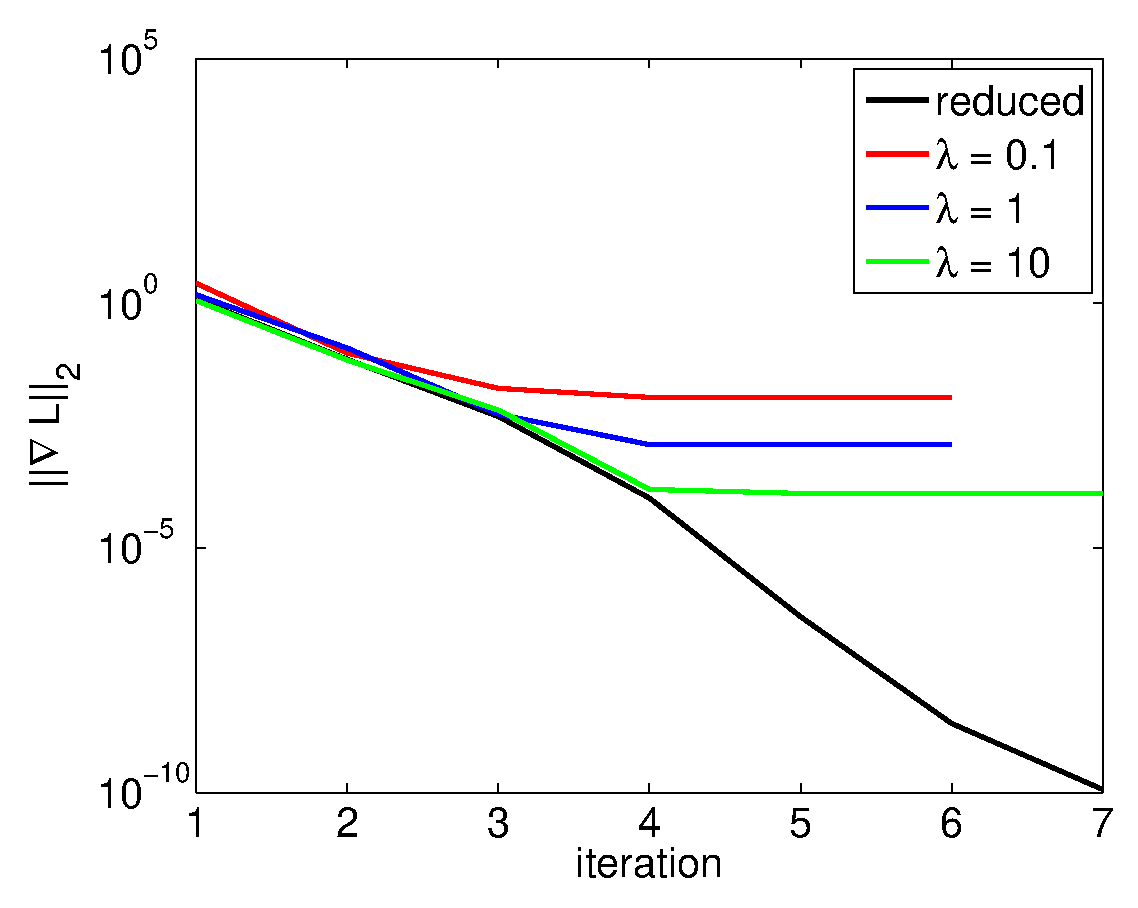
\includegraphics[scale=.4]{./figs/1D_exp1_a}&
\includegraphics[scale=.4]{./figs/1D_exp1_b}\\
{\small (a)}&{\small (b)}\\
\end{tabular}
\caption{Solutions and convergence history for 1D resisivity problem.}
\label{fig:1D_exp1}
\end{figure}

\begin{figure}
\centering
\begin{tabular}{cc}
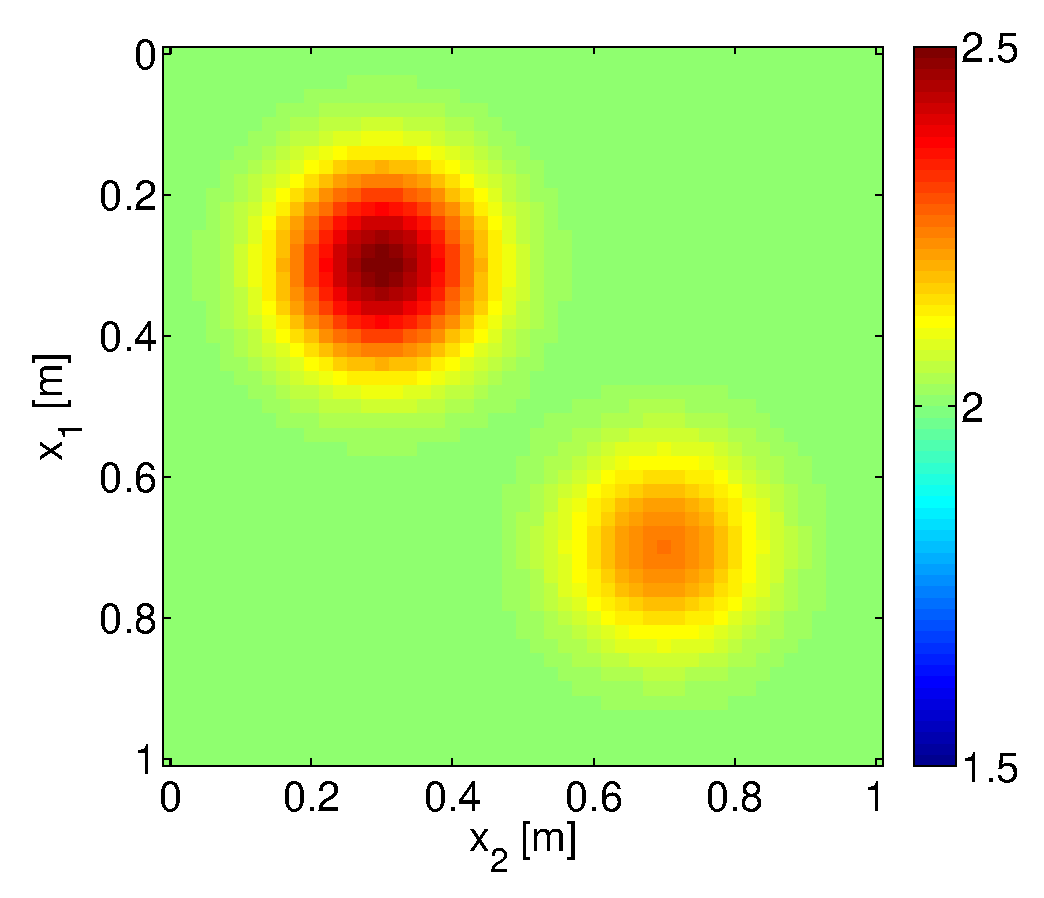
\includegraphics[scale=.4]{./figs/2D_exp1_a}&
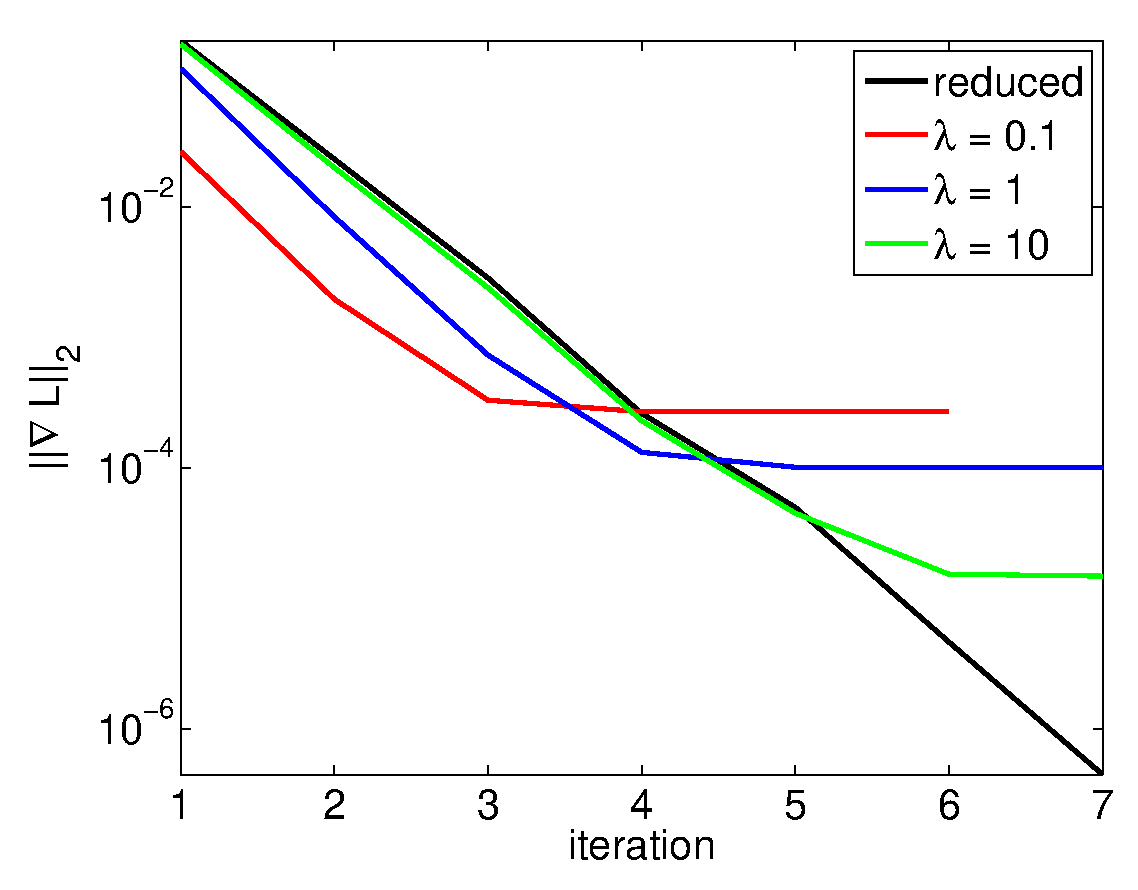
\includegraphics[scale=.4]{./figs/2D_exp1_b}\\
{\small (a)}&{\small (b)}\\
\end{tabular}
\caption{Sampling operator, ground truth and convergence history.}
\label{fig:2D_exp1a}
\end{figure}

\begin{figure}
\centering
\begin{tabular}{cccc}
\includegraphics[scale=.2]{./figs/2D_exp0_a}&
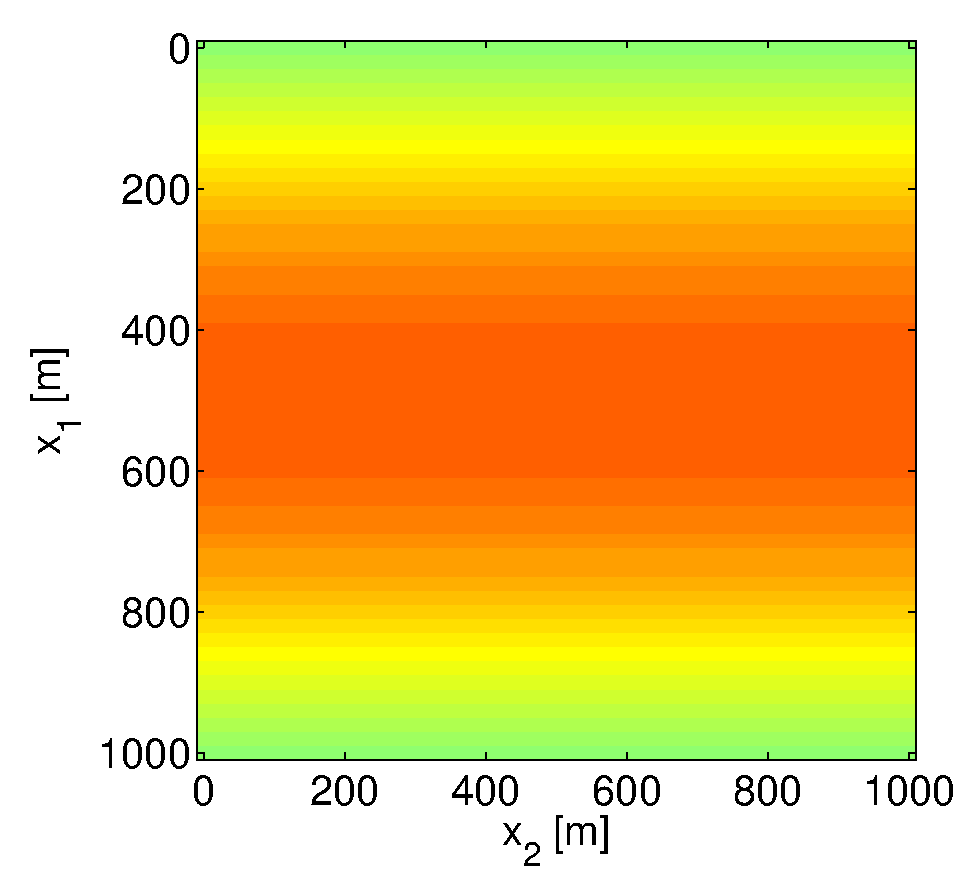
\includegraphics[scale=.2]{./figs/2D_exp0_b}&
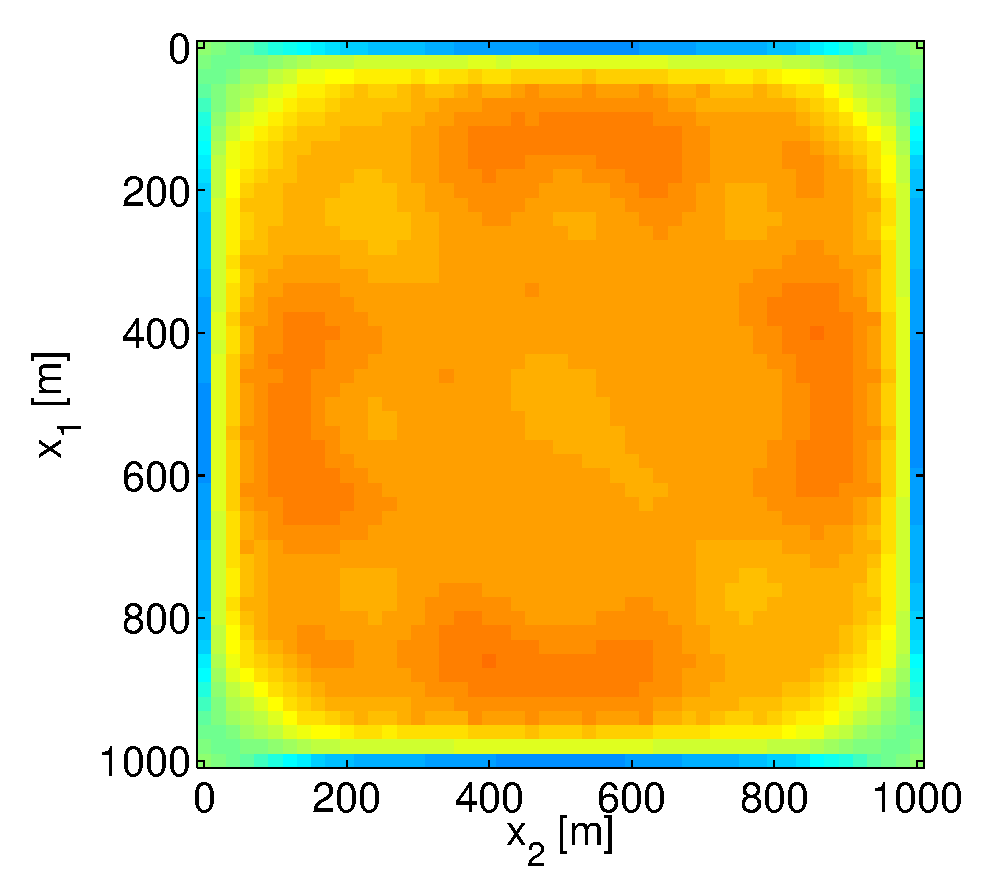
\includegraphics[scale=.2]{./figs/2D_exp0_c}&
\includegraphics[scale=.2]{./figs/2D_exp0_d}\\
\includegraphics[scale=.2]{./figs/2D_exp0_e}&
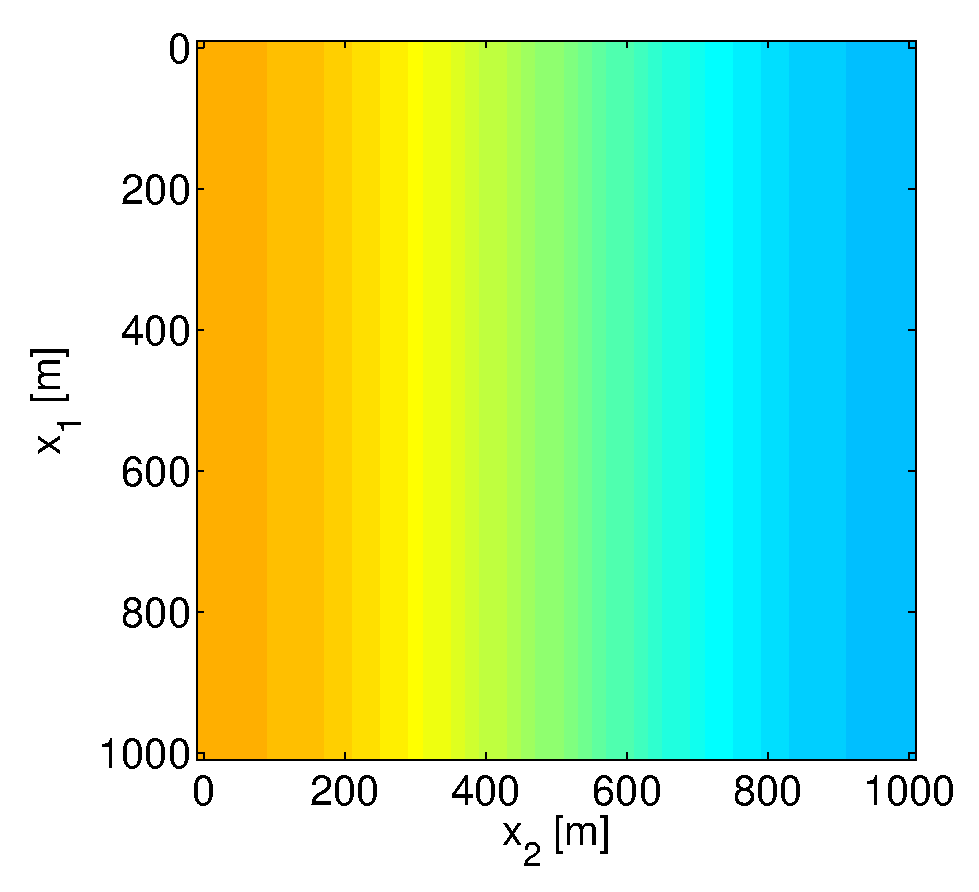
\includegraphics[scale=.2]{./figs/2D_exp0_f}&
\includegraphics[scale=.2]{./figs/2D_exp0_g}&
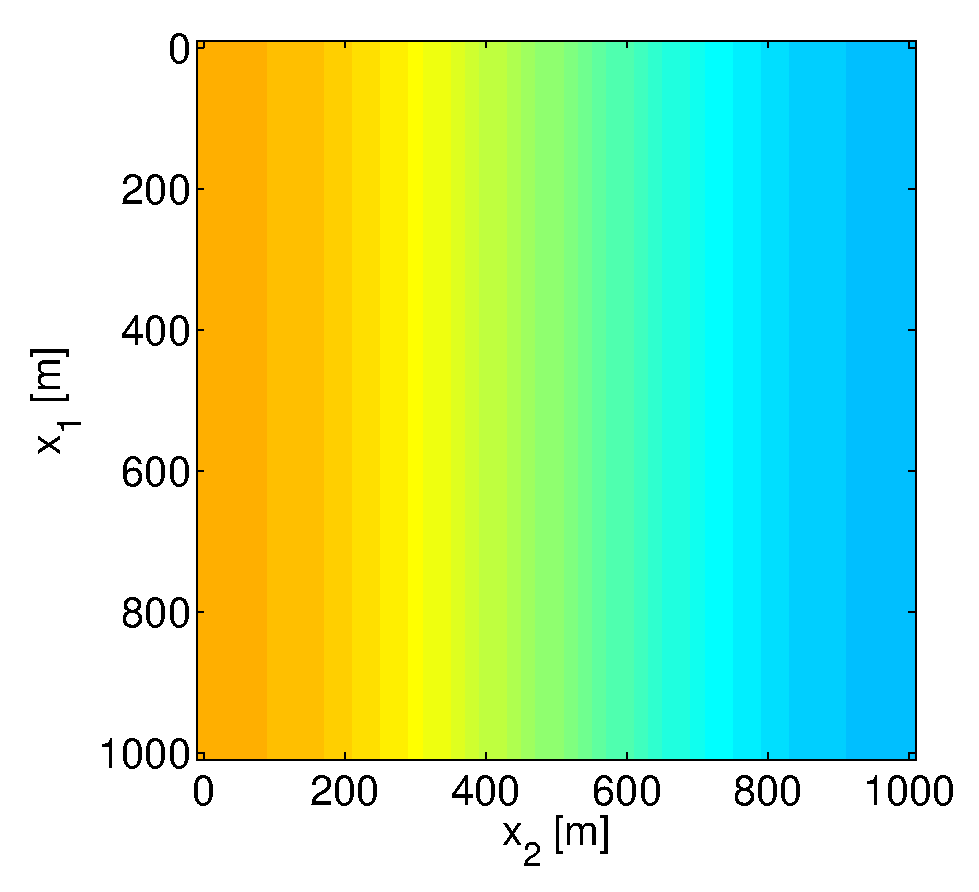
\includegraphics[scale=.2]{./figs/2D_exp0_h}\\
{\small reduced}&{\small $\lambda=0.1$}&{\small $\lambda=1$}&{\small $\lambda=10$}\\
\end{tabular}
\caption{Dominant eigenvectors of the GN Hessian.}
\label{fig:2D_exp0a}
\end{figure}

\begin{figure}
\centering
\begin{tabular}{cccc}
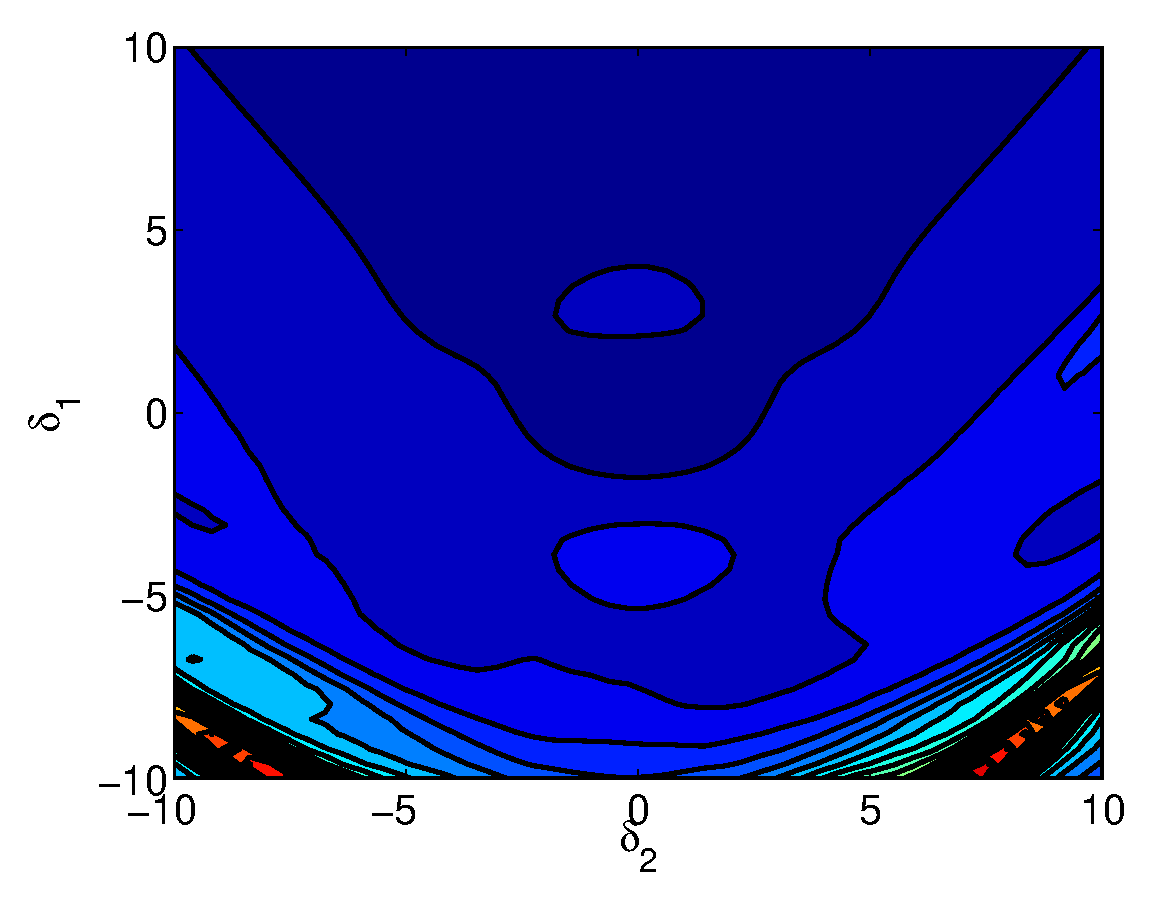
\includegraphics[scale=.2]{./figs/2D_exp0_i}&
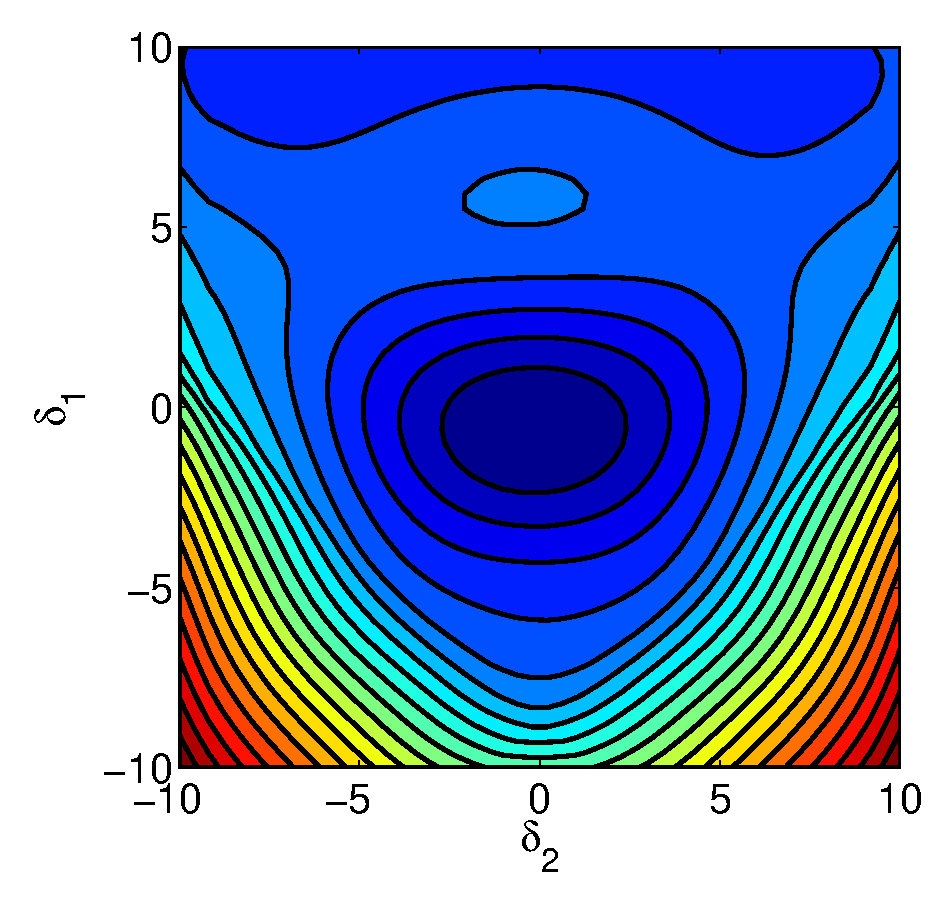
\includegraphics[scale=.2]{./figs/2D_exp0_j}&
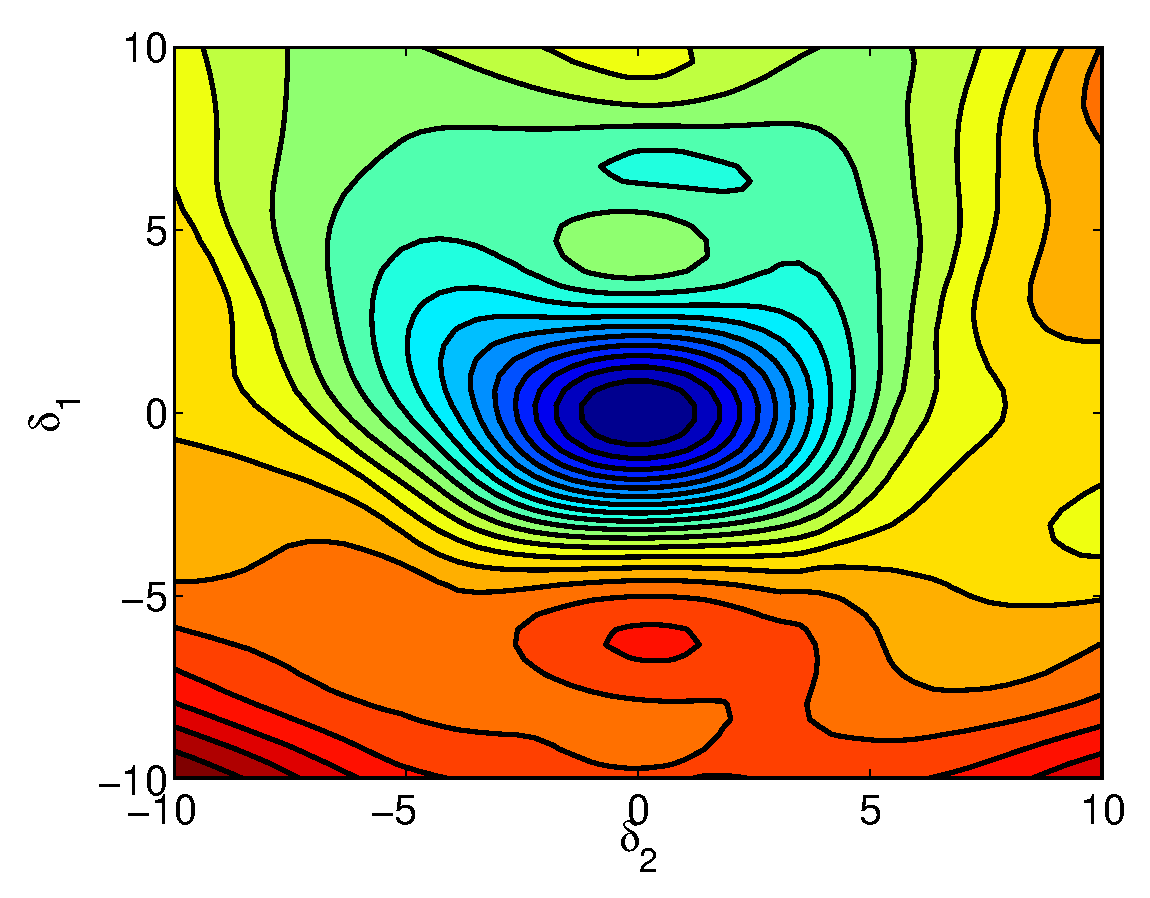
\includegraphics[scale=.2]{./figs/2D_exp0_k}&
\includegraphics[scale=.2]{./figs/2D_exp0_l}\\
{\small reduced}&{\small $\lambda=0.1$}&{\small $\lambda=1$}&{\small $\lambda=10$}\\
\end{tabular}
\caption{Misfit in the direction of the dominant eigenvector of the Hessian.}
\label{fig:2D_exp0b}
\end{figure}


\begin{figure}
\centering
\includegraphics[scale=.4]{./figs/2D_exp1_c}\\
\centering
\begin{tabular}{cccc}
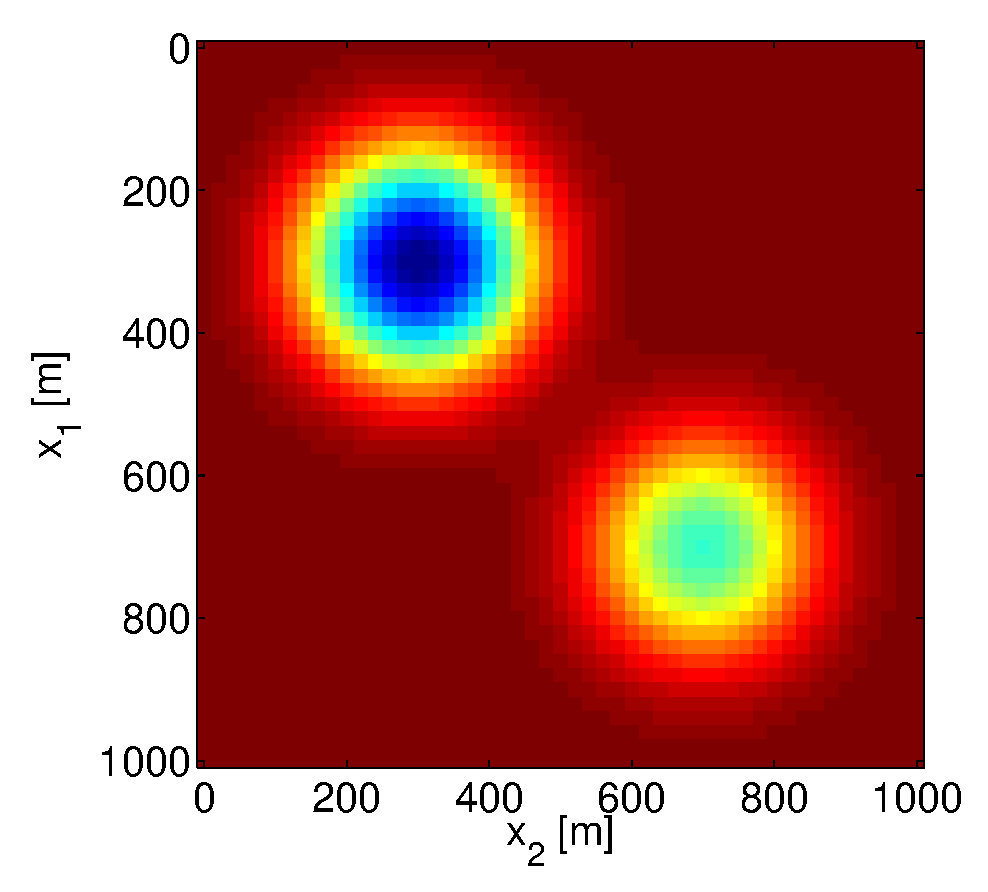
\includegraphics[scale=.2]{./figs/2D_exp1_d}&
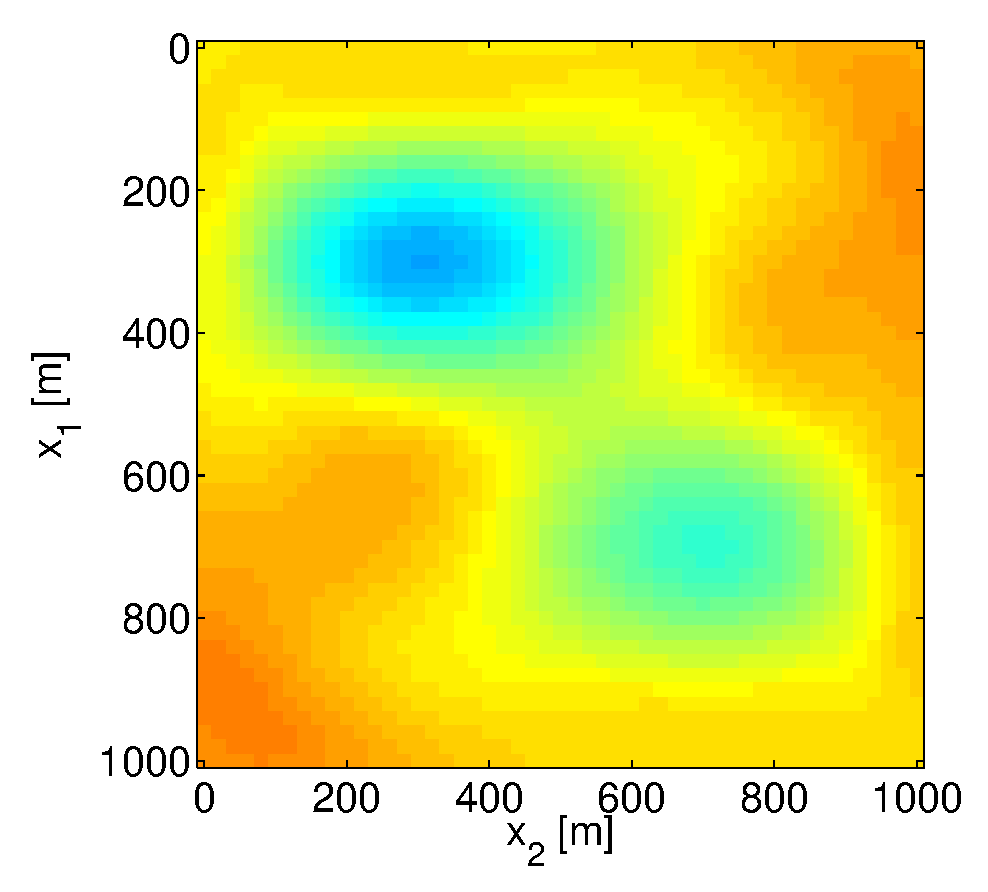
\includegraphics[scale=.2]{./figs/2D_exp1_e}&
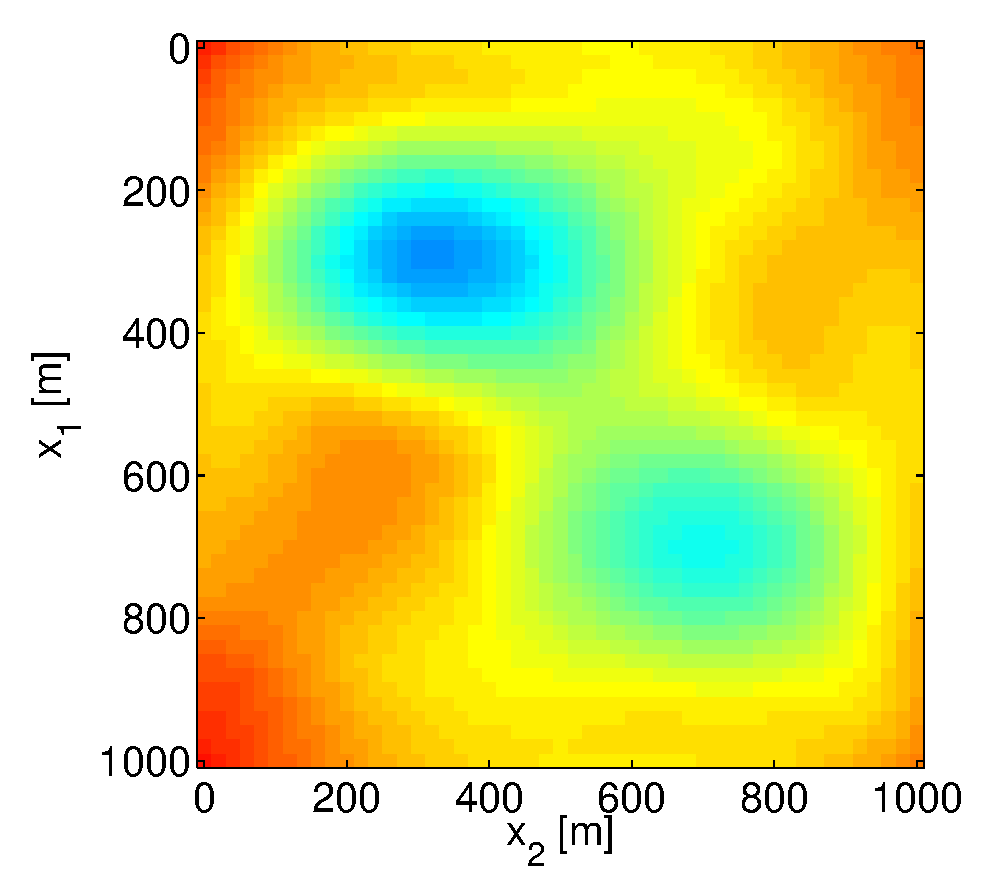
\includegraphics[scale=.2]{./figs/2D_exp1_f}&
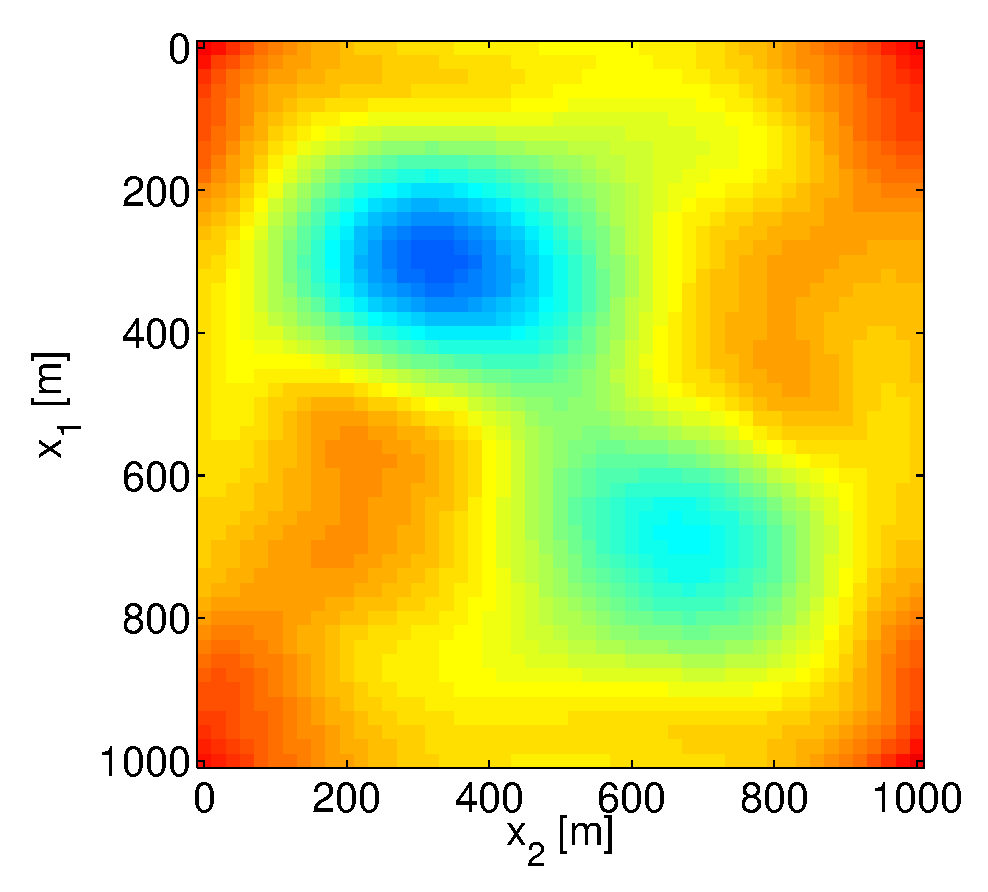
\includegraphics[scale=.2]{./figs/2D_exp1_g}\\
{\small reduced}&{\small $\lambda=0.1$}&{\small $\lambda=1$}&{\small $\lambda=10$}\\
\end{tabular}
\caption{Convergence history and reconstructions.}
\label{fig:2D_exp1b}
\end{figure}

\clearpage
\bibliographystyle{unsrt}
\bibliography{mybib}



\end{document}

